\documentclass[12pt,a4paper]{report}
\usepackage[margin=1in]{geometry}
\usepackage{amsmath,amssymb}
\usepackage{booktabs,array}
\usepackage{graphicx,float}
\usepackage{xcolor}
\usepackage{tikz}
\usepackage{enumitem}
\usepackage{fancyhdr}
\usepackage[hidelinks]{hyperref}
\usepackage{microtype}
\usepackage{caption,subcaption}
\usepackage{ragged2e}
% Report information
\newcommand{\studentname}{Sabbir Hossain}
\newcommand{\studentid}{21701082}
\newcommand{\session}{2020--2021}
\newcommand{\department}{Department of Computer Science and Engineering}
\newcommand{\university}{University of Chittagong}
\newcommand{\coursetitle}{Machine Learning Lab}
\newcommand{\coursecode}{CSE 816}
\newcommand{\instructor}{Prof. Dr. Mohammad Osir Rahman}
\newcommand{\submissiondate}{September 14, 2026}


\definecolor{darkgray}{HTML}{333333}
\definecolor{lightgray}{HTML}{EEEEEE}
\definecolor{headercolor}{HTML}{24527A}
\definecolor{tablecolor}{HTML}{EAF2F8}
\setlength{\parindent}{0pt}
\setlength{\parskip}{5pt}
\setlist{leftmargin=1.6em,itemsep=2pt,topsep=3pt}
\captionsetup{font=small,labelfont=bf}
\pagestyle{fancy}
\fancyhf{}
\fancyhead[L]{\coursecode: \coursetitle}
\fancyhead[R]{\studentid}
\fancyfoot[C]{\thepage}
\renewcommand{\headrulewidth}{0.4pt}

\newcommand{\experiment}[2]{
\chapter{#1}}

\begin{document}
\begin{titlepage}
\centering
\vspace*{0.5cm}

\IfFileExists{logo.png}{%
    \includegraphics[width=0.18\linewidth]{logo.png}\par
    \vspace{0.5cm}
}{}

{\Large\bfseries \university\par}
\vspace{0.2cm}
{\large \department\par}
\vspace{0.9cm}


\begin{tikzpicture}
\node[fill=headercolor!10,rounded corners=8pt,inner sep=15pt,
      text width=0.80\textwidth,align=center] {%
    {\LARGE\bfseries Machine Learning Lab Report}\\[0.35cm]
    {\large \coursecode: \coursetitle}
};
\end{tikzpicture}

\vspace{1.2cm}


\begin{tikzpicture}
\node[fill=tablecolor,rounded corners=6pt,inner sep=12pt,
      text width=0.70\textwidth,align=center] {%
    \textbf{Submitted To:}\\[0.2cm]
    \instructor\\
    \department\\
    \university
};
\end{tikzpicture}

\vspace{0.9cm}

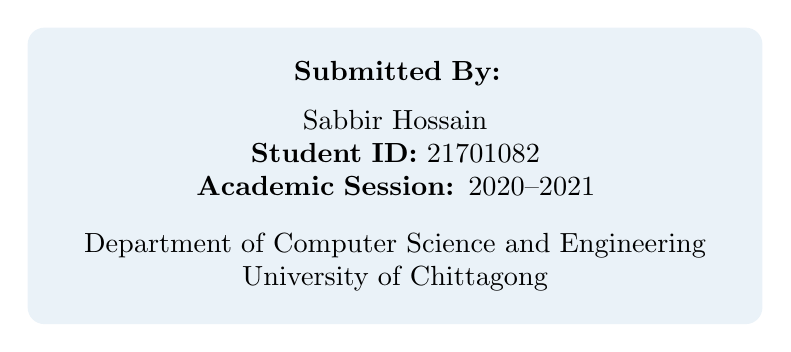
\begin{tikzpicture}
\node[fill=tablecolor,rounded corners=6pt,inner sep=12pt,
      text width=0.70\textwidth,align=center] {%
    \textbf{Submitted By:}\\[0.2cm]
    \studentname\\
    \textbf{Student ID:} \studentid\\
    \textbf{Academic Session:} \session\\[0.3cm]
    \department\\
    \university
};
\end{tikzpicture}

\vfill
{\large\textbf{Submission Date:} \submissiondate\par}
\thispagestyle{empty}
\end{titlepage}

\pagenumbering{roman}
\thispagestyle{plain}
\vspace*{\fill}
\begin{center}
{\LARGE\bfseries Abstract\par}
\vspace{0.5cm}
\begin{minipage}{0.85\textwidth}
\justifying
Five machine-learning experiments were implemented and evaluated: K-Means clustering, K-Nearest Neighbours classification, ID3 decision-tree classification, linear support-vector classification, and convolutional neural-network classification. The experiments covered unsupervised grouping, instance-based learning, information-gain-based tree induction, maximum-margin classification, and image feature learning. Data validation, appropriate preprocessing, model selection, held-out evaluation, and new-input prediction were included. The principal results were a WCSS of 8.525 for the two-cluster K-Means example, 82.50\% KNN test accuracy, 92.50\% decision-tree test accuracy, 100\% linear-SVM test accuracy, and 76.25\% CNN test accuracy on the selected CIFAR-10 classes. The results demonstrate the operation and limitations of each method rather than claiming equivalent suitability across tasks. The complete implementations are available in the \href{https://github.com/alphapie77/MachineLearningLab}{GitHub source-code repository}.
\end{minipage}
\end{center}
\vspace*{\fill}
\clearpage

\tableofcontents
\clearpage
\pagenumbering{arabic}

% ================================================================
\experiment{K-Means Clustering}{01}

\section{Objective}
To implement K-Means clustering for two-dimensional data, observe iterative centroid updates, evaluate cluster compactness using within-cluster sum of squares (WCSS), and assign a new point to a learned cluster.

\section{Introduction}
K-Means is an unsupervised algorithm: the data contain features but no target labels. Its purpose is to divide $n$ observations into $k$ groups so that observations within the same group are close to one another. Each group is represented by a centroid, which is the arithmetic mean of its member points.

For a point $x_i$ and centroid $\mu_j$, Euclidean distance is
\begin{equation}
d(x_i,\mu_j)=\sqrt{\sum_{m=1}^{p}(x_{im}-\mu_{jm})^2}.
\end{equation}
The point is assigned to the nearest centroid,
\begin{equation}
c_i=\arg\min_j \lVert x_i-\mu_j\rVert_2,
\end{equation}
after which centroid $j$ is updated as
\begin{equation}
\mu_j=\frac{1}{|C_j|}\sum_{x_i\in C_j}x_i.
\end{equation}
Assignment and update are repeated until neither the assignments nor centroids change. WCSS measures the remaining spread:
\begin{equation}
\mathrm{WCSS}=\sum_{j=1}^{k}\sum_{x_i\in C_j}\lVert x_i-\mu_j\rVert_2^2.
\end{equation}
Here, $p$ is the number of features, $C_j$ is the set of points assigned to cluster $j$, and $|C_j|$ is the number of points in that cluster. A smaller WCSS means that points lie closer to their centroids. Since WCSS normally decreases as $k$ increases, the elbow method looks for a bend after which the improvement becomes comparatively small.

For example, the distance from $(2,3)$ to centroids $(1,1)$ and $(5,7)$ is $\sqrt5\approx2.236$ and $5$, respectively; therefore, the point joins the first cluster. This same calculation is applied to every row.

\section{Materials and Method}
\textbf{Software:} Python 3.13.3, Tkinter, Matplotlib 3.11.2, and the supplied K-Means implementation. The dataset contained seven samples with an ID and two numerical features, $x$ and $y$. ID was used only to identify rows.

The following procedure was used:
\begin{enumerate}
\item The CSV file was loaded and checked for missing, non-numeric, or non-finite coordinates.
\item The number of clusters was set to $k=2$. Initial centroids $(1,1)$ and $(5,7)$ were obtained by deterministic farthest-point initialisation.
\item Euclidean distances were calculated and each point was assigned to its nearest centroid.
\item New centroids were calculated from cluster means. The process continued until convergence.
\item WCSS was calculated for $k=1$ to $6$ to form an elbow curve.
\item A new input point was assigned to the nearest final centroid without retraining.
\end{enumerate}

\section{Results}
The algorithm converged after three iterations. The final centroids were $(1.25,1.50)$ and $(3.90,5.10)$, with WCSS $=8.525$.

\begin{table}[H]\centering
\caption{WCSS obtained for candidate numbers of clusters}
\begin{tabular}{ccccccc}\toprule
$k$&1&2&3&4&5&6\\\midrule
WCSS&37.071&8.525&2.500&1.292&0.667&0.125\\\bottomrule
\end{tabular}\end{table}

\begin{figure}[H]\centering
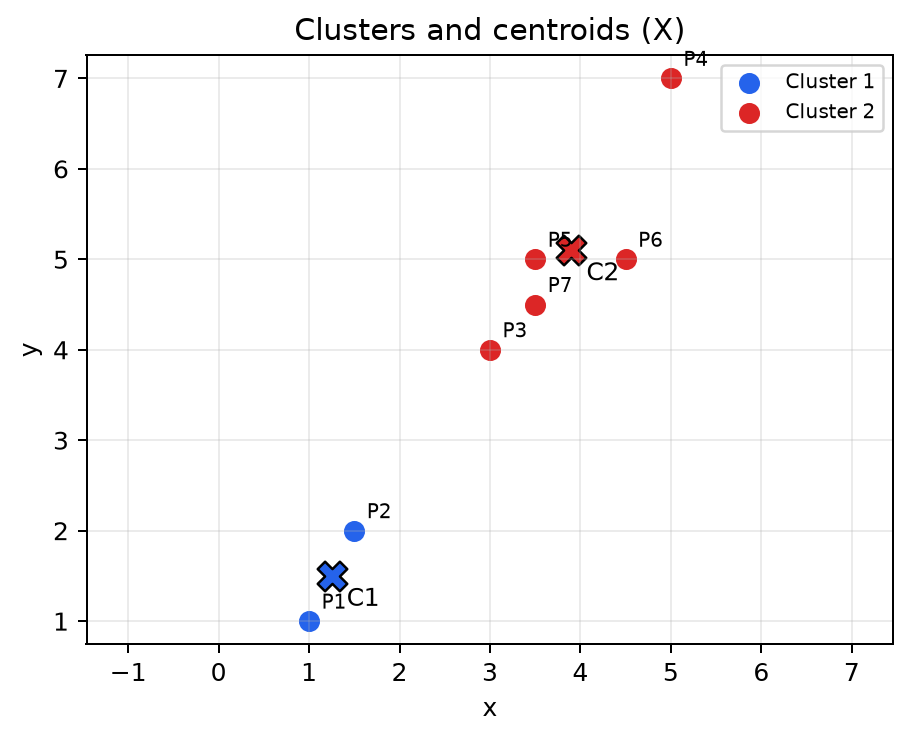
\includegraphics[width=0.80\textwidth]{figures/kmeans_clusters.png}
\caption{Final cluster assignments and learned centroids.}
\label{fig:kmeansclusters}
\end{figure}

\begin{figure}[H]\centering
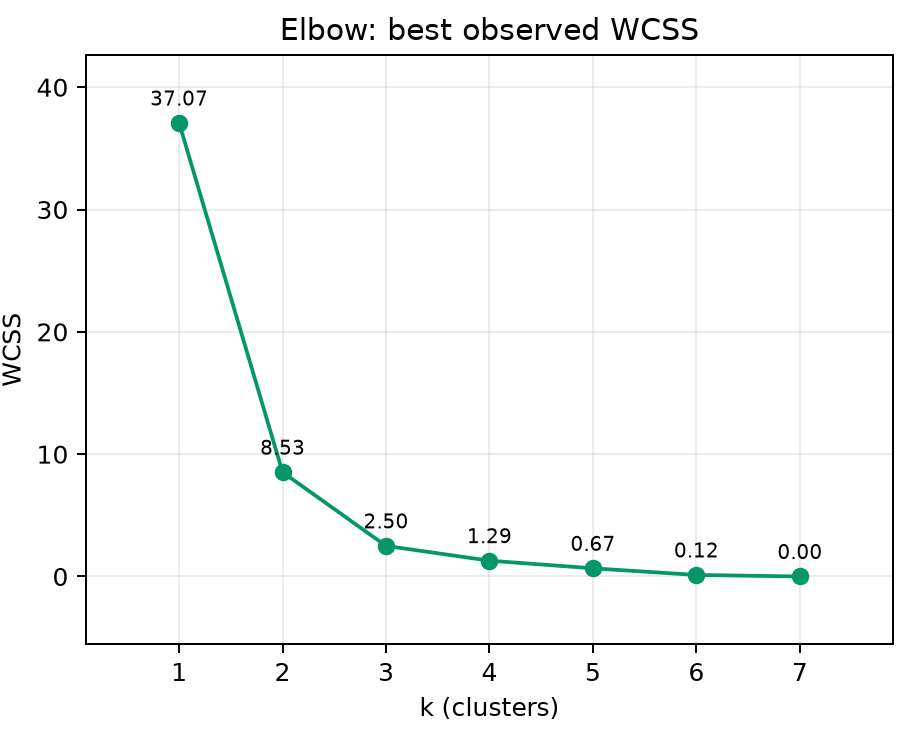
\includegraphics[width=0.80\textwidth]{figures/kmeans_elbow.png}
\caption{WCSS elbow curve generated by the program.}
\label{fig:kmeanselbow}
\end{figure}

\section{Discussion}
Figure~\ref{fig:kmeansclusters} shows compact groups around the two final centroids. Figure~\ref{fig:kmeanselbow} shows that WCSS decreased sharply from 37.071 at $k=1$ to 8.525 at $k=2$, confirming that a single centroid represented the data poorly. WCSS continued to decrease for larger $k$ because additional centroids can only maintain or reduce within-cluster distances; therefore, the smallest WCSS must not be selected automatically. The elbow indicates the point where additional clusters provide diminishing practical improvement.

The method is sensitive to feature scale and initial centroids. It also represents groups through means and Euclidean distances, so elongated or irregularly shaped clusters may not be modelled well. Accuracy and confusion matrices were not reported because no true class labels existed.

\section{Conclusion}
K-Means successfully divided the example data into two clusters and converged to centroids $(1.25,1.50)$ and $(3.90,5.10)$. The distance table, centroid updates, WCSS, elbow curve, and new-point assignment verified the complete clustering process.

% ================================================================
\experiment{K-Nearest Neighbours Classification}{02}

\section{Objective}
To classify shirt size from height and weight using KNN, select $k$ without test-data leakage, and evaluate performance in the presence of class imbalance.

\section{Introduction}
KNN is a supervised, non-parametric, instance-based classifier. It stores the training observations rather than estimating an explicit equation. For a new input, distances to the training samples are calculated, the nearest $k$ samples are selected, and their labels vote for the output class.

``Supervised'' means that every training row has a known output label, while ``instance-based'' means that a query is compared directly with stored examples. Here, height and weight were the two inputs, and shirt size L or M was the output.

Because height and weight have different distributions, they were standardised using training-set statistics:
\begin{equation}
z=\frac{x-\mu_{\mathrm{train}}}{\sigma_{\mathrm{train}}}.
\end{equation}
For example, if the three nearest neighbours have labels M, M, and L, then $k=3$ produces two votes for M and one for L; the predicted class is M. A small $k$ can be sensitive to noise, while an excessively large $k$ can favour the majority class. Cross-validation was therefore used to select $k$.

\section{Materials and Method}
\textbf{Software:} Python 3.13.3, Tkinter, Matplotlib 3.11.2, and the supplied KNN implementation. The dataset contained 1,000 observations with height (cm), weight (kg), and shirt-size label. Class counts were M$=835$ and L$=165$.

The data were divided into a stratified 80\% training partition and a 20\% test partition. Candidate values $k\in\{3,5,7,9\}$ were compared by five-fold cross-validation using only the training partition. Within each fold, standardisation parameters were fitted on the fold's training rows and then applied to its validation rows. Mean macro-F1 selected $k$, giving equal importance to M and L. The final scaler and KNN model were then evaluated once on the untouched test partition. For a user input, the application displayed the scaled query, nearest samples, distances, votes, and predicted size.

Precision describes how often predictions of a class were correct, recall describes how many actual members of that class were found, and F1 combines precision and recall. A macro score averages the separate L and M scores, preventing the larger class from dominating. ROC--AUC evaluates how well the vote score ranks the classes across different thresholds; 0.5 represents chance-level ranking and 1.0 represents perfect ranking.

\section{Results}
The selected value was $k=7$. Table~\ref{tab:knnmetrics} summarises the held-out test results. Figures~\ref{fig:knnconfusion} and~\ref{fig:knnroc} present the confusion matrix and ROC curve separately.

\begin{table}[H]\centering
\caption{KNN performance on 200 test observations}\label{tab:knnmetrics}
\begin{tabular}{lc}\toprule
Measure&Value\\\midrule
Accuracy&82.50\%\\
Macro precision&63.39\%\\
Macro recall (balanced accuracy)&55.48\%\\
Macro F1&56.18\%\\
ROC--AUC&0.6614\\\bottomrule
\end{tabular}\end{table}

\begin{table}[H]\centering
\caption{KNN confusion matrix}\label{tab:knncm}
\begin{tabular}{lcc}\toprule
&Predicted L&Predicted M\\\midrule
Actual L&5&28\\
Actual M&7&160\\\bottomrule
\end{tabular}\end{table}

\begin{figure}[H]\centering
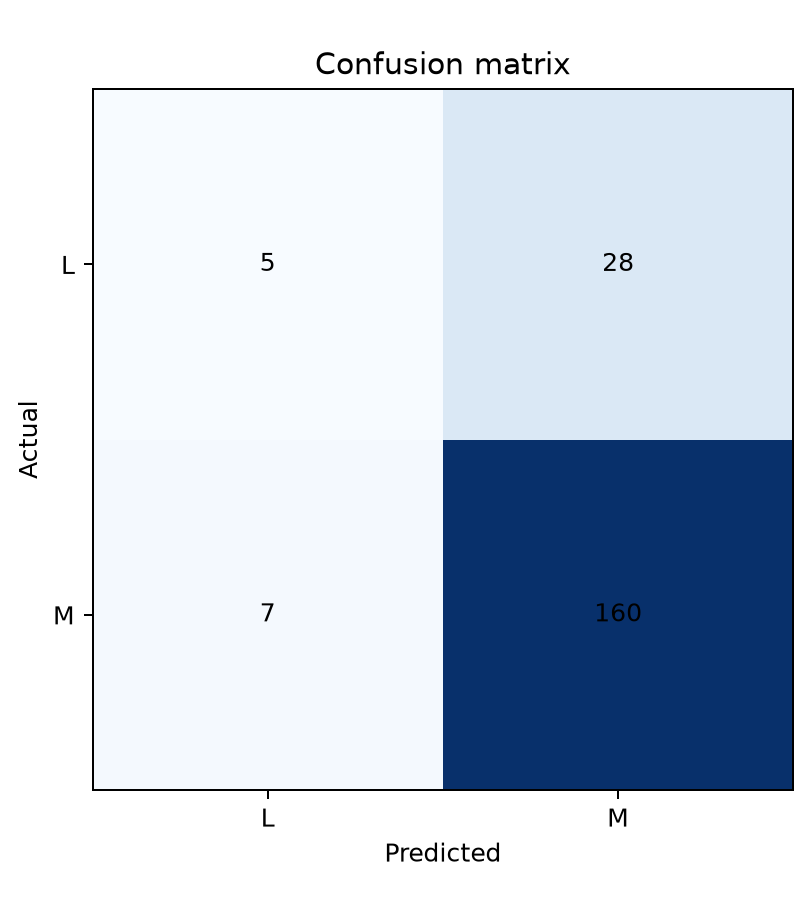
\includegraphics[width=0.80\textwidth]{figures/knn_confusion.png}
\caption{KNN confusion matrix computed from the untouched test partition.}
\label{fig:knnconfusion}
\end{figure}

\begin{figure}[H]\centering
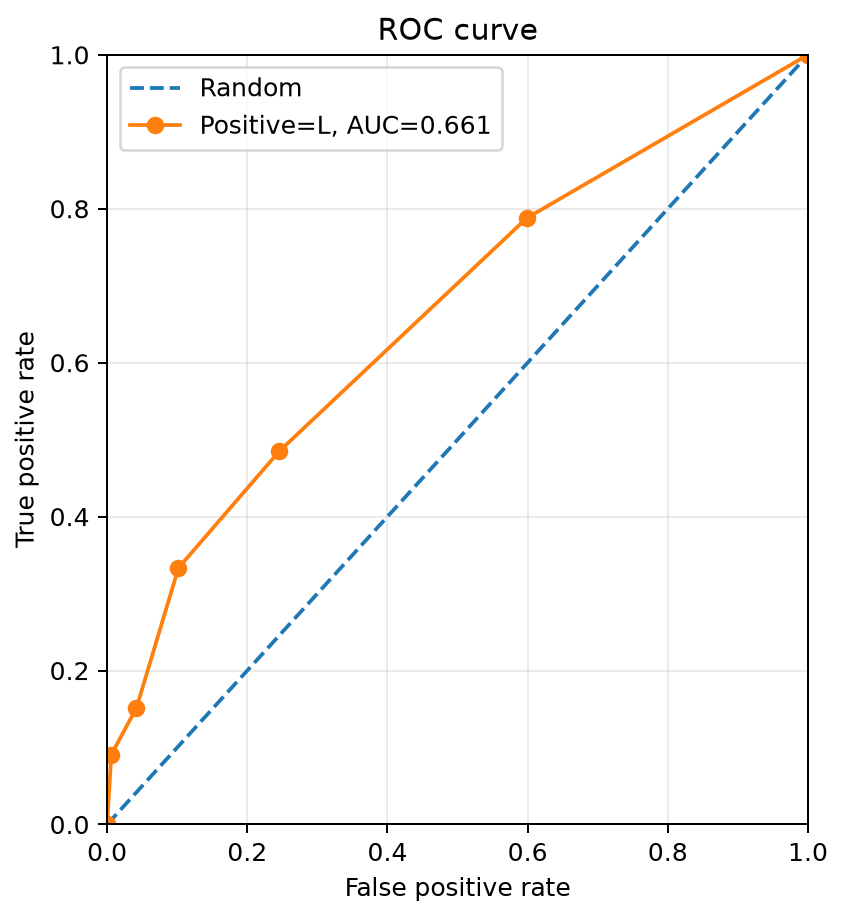
\includegraphics[width=0.80\textwidth]{figures/knn_roc.png}
\caption{KNN ROC curve computed from the untouched test partition.}
\label{fig:knnroc}
\end{figure}

\section{Discussion}
The overall accuracy of 82.50\% appears reasonable, but Table~\ref{tab:knncm} shows that only 5 of 33 L observations were correctly classified, compared with 160 of 167 M observations. The class imbalance therefore made accuracy optimistic. Macro recall of 55.48\% and macro F1 of 56.18\% describe this weakness more clearly. The ROC--AUC of 0.6614 indicates only moderate ranking ability for the minority class.

The confusion-matrix rows are the true labels and the columns are the predictions. Thus, 28 means that 28 actual L shirts were incorrectly predicted as M; this was the main error.

The experiment shows why both the data distribution and class-specific results must be examined. Possible improvements include collecting more L examples, distance-weighted voting, or resampling. KNN also requires distance calculations at prediction time, which becomes costly for large training sets.

\section{Conclusion}
The KNN implementation correctly applied stratified splitting, training-only standardisation, cross-validated selection of $k$, held-out evaluation, and transparent neighbour voting. The results also demonstrated that accuracy alone is inadequate for this imbalanced dataset.

% ================================================================
\experiment{ID3 Decision Tree Classification}{03}

\section{Objective}
To construct an ID3 tree from categorical weather data, select tree depth using training-only cross-validation, evaluate its predictions, and trace decisions from the root to a leaf.

\section{Introduction}
A decision tree predicts by asking a sequence of feature questions. ID3 chooses each question using entropy and information gain. For class proportions $p_i$, entropy is
\begin{equation}
H(S)=-\sum_i p_i\log_2p_i.
\end{equation}
Entropy equals zero when all labels agree and reaches one for two equally common classes. If a feature $A$ divides $S$ into subsets $S_v$, its information gain is
\begin{equation}
IG(S,A)=H(S)-\sum_{v\in Values(A)}\frac{|S_v|}{|S|}H(S_v).
\end{equation}
The feature producing the greatest reduction in uncertainty becomes the current node. The procedure is repeated on each branch until a leaf or stopping condition is reached.

A root is the first question, a branch is one possible answer, and a leaf is the final prediction. For example, Figure~\ref{fig:tree} predicts No for Outlook=Sunny and Humidity=High by following the Sunny branch and then the High branch.

\section{Materials and Method}
\textbf{Software:} Python 3.13.3, Tkinter, Matplotlib 3.11.2, and the supplied ID3 implementation. The dataset contained 1,000 categorical weather records and a binary target named \texttt{Play}.

A reproducible stratified 80/20 split produced training and test partitions. Five-fold cross-validation on the training partition compared maximum depths 1--5. The selected depth was used to train the final tree on all training rows. Accuracy, precision, recall, F1, ROC--AUC, and a confusion matrix were calculated from the untouched test rows. New inputs were entered through feature dropdowns; the application returned both a class and its root-to-leaf path. Unseen categories used the majority label stored at the current node instead of causing failure. For the binary metrics, Yes was treated as the positive class; precision therefore describes Yes predictions, while recall describes the proportion of actual Yes cases found.

\section{Results}
Cross-validation selected maximum depth 2. The learned tree used \texttt{Outlook} at the root. Overcast and Rainy branches tested \texttt{Wind}; the Sunny branch tested \texttt{Humidity}. Table~\ref{tab:dtmetrics} reports test performance, and Figure~\ref{fig:tree} shows the fitted tree.

\begin{table}[H]\centering
\caption{ID3 performance on the test partition}\label{tab:dtmetrics}
\begin{tabular}{lc}\toprule
Measure&Value\\\midrule
Selected maximum depth&2\\
Accuracy&92.50\%\\
Precision&93.80\%\\
Recall&94.53\%\\
F1-score&94.16\%\\
ROC--AUC&92.89\%\\
Leaves&6\\\bottomrule
\end{tabular}\end{table}

\begin{figure}[H]\centering
\resizebox{0.80\textwidth}{!}{%
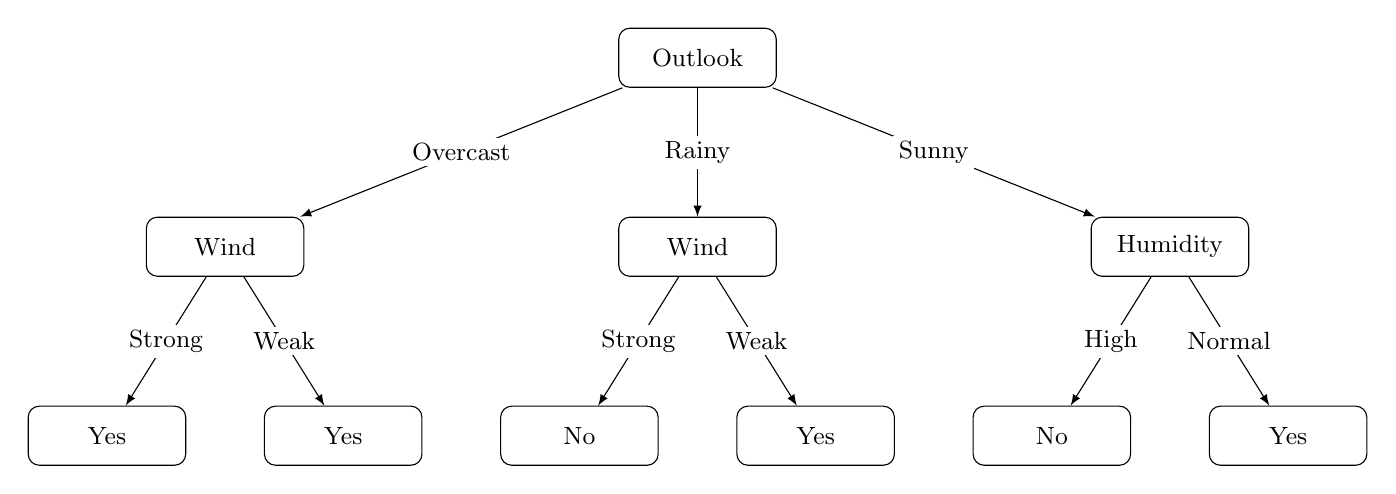
\begin{tikzpicture}[
box/.style={draw,rounded corners,align=center,font=\small,minimum width=2.0cm,minimum height=0.75cm},
edgeLabel/.style={fill=white,inner sep=2pt,font=\small}]
\node[box] (root) at (0,4.8) {Outlook};
\node[box] (overcast) at (-6,2.4) {Wind};
\node[box] (rainy) at (0,2.4) {Wind};
\node[box] (sunny) at (6,2.4) {Humidity};

\node[box] (oyes1) at (-7.5,0) {Yes};
\node[box] (oyes2) at (-4.5,0) {Yes};
\node[box] (rno) at (-1.5,0) {No};
\node[box] (ryes) at (1.5,0) {Yes};
\node[box] (sno) at (4.5,0) {No};
\node[box] (syes) at (7.5,0) {Yes};

\draw[-latex] (root) -- node[edgeLabel] {Overcast} (overcast);
\draw[-latex] (root) -- node[edgeLabel] {Rainy} (rainy);
\draw[-latex] (root) -- node[edgeLabel] {Sunny} (sunny);
\draw[-latex] (overcast) -- node[edgeLabel] {Strong} (oyes1);
\draw[-latex] (overcast) -- node[edgeLabel] {Weak} (oyes2);
\draw[-latex] (rainy) -- node[edgeLabel] {Strong} (rno);
\draw[-latex] (rainy) -- node[edgeLabel] {Weak} (ryes);
\draw[-latex] (sunny) -- node[edgeLabel] {High} (sno);
\draw[-latex] (sunny) -- node[edgeLabel] {Normal} (syes);
\end{tikzpicture}
}
\caption{Depth-two ID3 tree learned from the training partition.}
\label{fig:tree}
\end{figure}

\section{Discussion}
The compact tree in Figure~\ref{fig:tree} explains each prediction through at most two feature tests. The 92.50\% accuracy and 94.16\% F1-score show that the selected tree generalised well without unnecessary depth. Selecting depth only on training folds prevented the final test rows from influencing model complexity.

Decision trees are easy to interpret but can change substantially when the data change. ID3 may also favour categorical features with many possible values. Depth control reduced overfitting in this experiment, but larger or noisier data may require additional pruning.

\section{Conclusion}
The experiment verified entropy, information gain, recursive tree induction, cross-validated depth selection, held-out evaluation, and explainable new-input prediction. The learned depth-two tree achieved 92.50\% test accuracy.

% ================================================================
\experiment{Linear Support Vector Machine}{04}

\section{Objective}
To implement a linear soft-margin SVM using Pegasos optimisation, select the regularisation parameter $C$, visualise the separating hyperplane and margins, and evaluate binary classification.

\section{Introduction}
A linear SVM predicts from the decision function
\begin{equation}
f(x)=w^Tx+b, \qquad \hat y=\begin{cases}+1,&f(x)\ge0,\\-1,&f(x)<0.\end{cases}
\end{equation}
Rather than selecting any separating line, SVM seeks a boundary with a large margin. Points on or inside the margin are support vectors and have the greatest influence on the boundary. The soft-margin objective is
\begin{equation}
J(w,b)=\frac12\lVert w\rVert^2+C\sum_i\max\left(0,1-y_i(w^Tx_i+b)\right).
\end{equation}
The first term favours a wide margin and the hinge-loss term penalises violations. Parameter $C$ controls their trade-off. Pegasos uses stochastic sub-gradient updates to minimise this objective.

The central line $w^Tx+b=0$ is the decision boundary, while $w^Tx+b=+1$ and $w^Tx+b=-1$ are the margin lines. The sign of $f(x)$ selects the class, and $|f(x)|$ reflects how far the point lies from the boundary in decision-score units.

As a numerical example, if $w=(2,-1)$, $b=-0.5$, and $x=(3,1)$, then $f(x)=2(3)-1(1)-0.5=4.5$ and the predicted class is $+1$.

\section{Materials and Method}
\textbf{Software:} Python 3.13.3, NumPy 2.5.3, Tkinter, Matplotlib 3.11.2, and the supplied Pegasos implementation. The synthetic dataset contained 500 two-dimensional samples labelled $-1$ or $+1$.

A stratified split produced 400 training and 100 test samples. Standardisation parameters were estimated only from training data. Five-fold cross-validation compared $C\in\{0.01,0.1,1,10,100\}$. The final Pegasos model was trained on the complete standardised training partition using the selected $C$. Hard predictions were used for the confusion matrix and class metrics; continuous decision scores were used for ROC--AUC. An ROC curve plots true-positive rate against false-positive rate as the threshold changes, while its area summarises ranking performance. A new point was standardised with stored training statistics before its decision score was calculated.

\section{Results}
Cross-validation selected $C=0.01$. All 100 test observations were classified correctly, as reported in Table~\ref{tab:svmmetrics}. The fitted boundary and margins are shown in Figure~\ref{fig:svmboundary}, while Figure~\ref{fig:svmroc} presents the ROC curve.

\begin{table}[H]\centering
\caption{Linear SVM test results}\label{tab:svmmetrics}
\begin{tabular}{lc}\toprule
Measure&Value\\\midrule
Accuracy&100\%\\
Precision&100\%\\
Recall&100\%\\
F1-score&100\%\\
ROC--AUC&1.000\\
$(TP,FP,FN,TN)$&$(50,0,0,50)$\\\bottomrule
\end{tabular}\end{table}

\begin{figure}[H]\centering
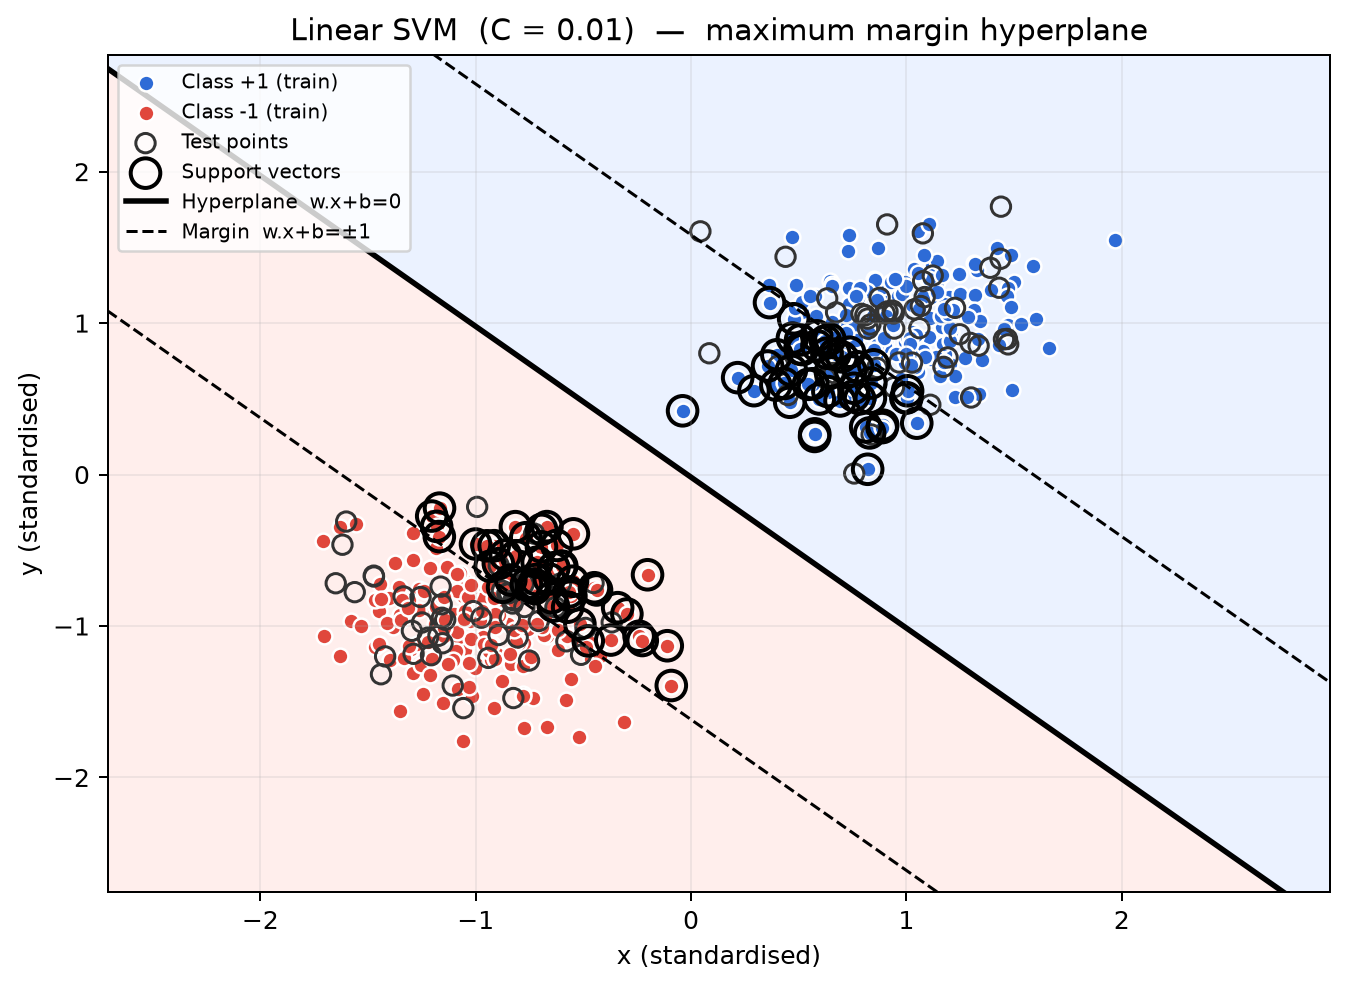
\includegraphics[width=0.80\textwidth]{figures/linear_boundary.png}
\caption{Decision boundary and margins of the trained linear SVM.}
\label{fig:svmboundary}
\end{figure}

\begin{figure}[H]\centering
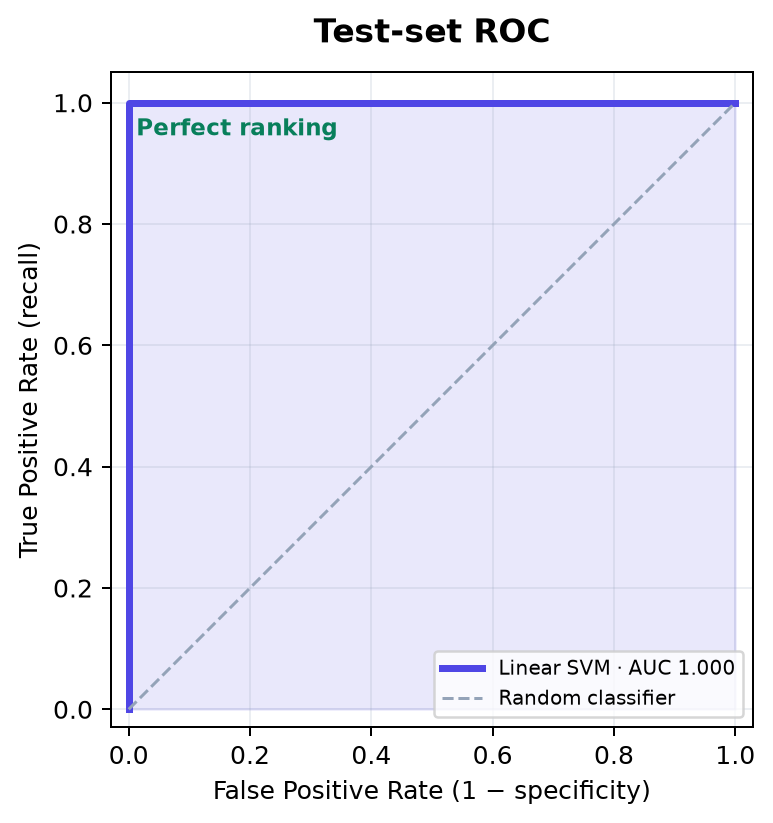
\includegraphics[width=0.80\textwidth]{figures/linear_roc.png}
\caption{Test-set ROC curve of the trained linear SVM.}
\label{fig:svmroc}
\end{figure}

\section{Discussion}
The classes in the synthetic dataset were linearly separable. Consequently, the confusion matrix contained no errors. The ROC curve rose vertically from $(0,0)$ to $(0,1)$ and then horizontally to $(1,1)$, producing AUC 1.000. This L shape is correct: every positive test observation received a higher decision score than every negative observation.

Perfect performance on this controlled dataset does not imply perfect performance on arbitrary data. Overlap, noise, outliers, or a non-linear class boundary would reduce the scores. The experiment is therefore evidence that the implementation works on a linearly separable problem, not that a linear SVM is universally sufficient.

\section{Conclusion}
The Pegasos SVM successfully learned a maximum-margin linear classifier with $C=0.01$. Training-only preprocessing, cross-validated model selection, margin visualisation, decision-score prediction, and test evaluation were verified.

% ================================================================
\experiment{CNN-Based Cat--Dog Image Classification}{05}

\section{Objective}
To train a convolutional neural network for binary cat--dog classification, evaluate it on unseen CIFAR-10 images, and classify consecutive user-supplied images.

\section{Introduction}
An RGB image is an array of pixel values with height, width, and three colour channels. A convolutional neural network learns small filters that slide over local image regions. Early feature maps can respond to edges and colour changes; deeper maps combine them into more complex visual patterns.

For filter $k$, a convolutional output is
\begin{equation}
Z_{i,j,k}=\sum_{u,v,c}W_{u,v,c,k}X_{i+u,j+v,c}+b_k.
\end{equation}
ReLU supplies non-linearity, max-pooling reduces spatial resolution, and dropout reduces co-adaptation during training. The final sigmoid produces
\begin{equation}
P(\mathrm{Dog}\mid x)=\frac{1}{1+e^{-z}}.
\end{equation}
The class is Dog when this probability is at least 0.5; otherwise it is Cat. Binary cross-entropy penalises disagreement between the target $y$ and probability $p$:
\begin{equation}
\mathcal L=-\frac1n\sum_i\left[y_i\log p_i+(1-y_i)\log(1-p_i)\right].
\end{equation}
Cat was encoded as 0 and Dog as 1, so the sigmoid value is the estimated Dog probability. For a Cat prediction, displayed confidence is $1-P(\mathrm{Dog}\mid x)$; for a Dog prediction, it is $P(\mathrm{Dog}\mid x)$.

\section{Materials and Method}
\textbf{Software:} Python 3.13.3, TensorFlow 2.21.0/Keras, NumPy 2.5.3, Pillow 12.3.0, Tkinter, and Matplotlib 3.11.2. CIFAR-10 contains 60,000 $32\times32$ RGB images in ten classes. Only class 3 (cat) and class 5 (dog) were selected. This provided 10,000 development images and 2,000 official test images.

Pixels were converted to \texttt{float32} and divided by 255. The development images were shuffled reproducibly and divided into training and validation subsets. The network contained Conv2D(32), max-pooling, Conv2D(64), max-pooling, flattening, Dense(64), Dropout(0.3), and a sigmoid output. Adam minimised binary cross-entropy. Early stopping monitored validation loss with patience three and restored the best weights. The official test set was used only after training decisions were complete.

For external input, the image was opened, converted to RGB, resized to $32\times32$, and normalised. Corrupt files and images smaller than $8\times8$ were rejected. The interface cleared the previous result before predicting another image and displayed the active filename.

\section{Results}
The saved network contained 166,977 trainable parameters. On the 2,000-image official cat/dog test subset, loss was 0.4940 and accuracy was 76.25\%. Table~\ref{tab:cnncm} and Figure~\ref{fig:cnncm} present the class-level test outcomes.

\begin{table}[H]\centering
\caption{CNN confusion matrix on the official test subset}\label{tab:cnncm}
\begin{tabular}{lcc}\toprule
&Predicted Cat&Predicted Dog\\\midrule
Actual Cat&733&267\\
Actual Dog&208&792\\\bottomrule
\end{tabular}\end{table}

\begin{figure}[H]\centering
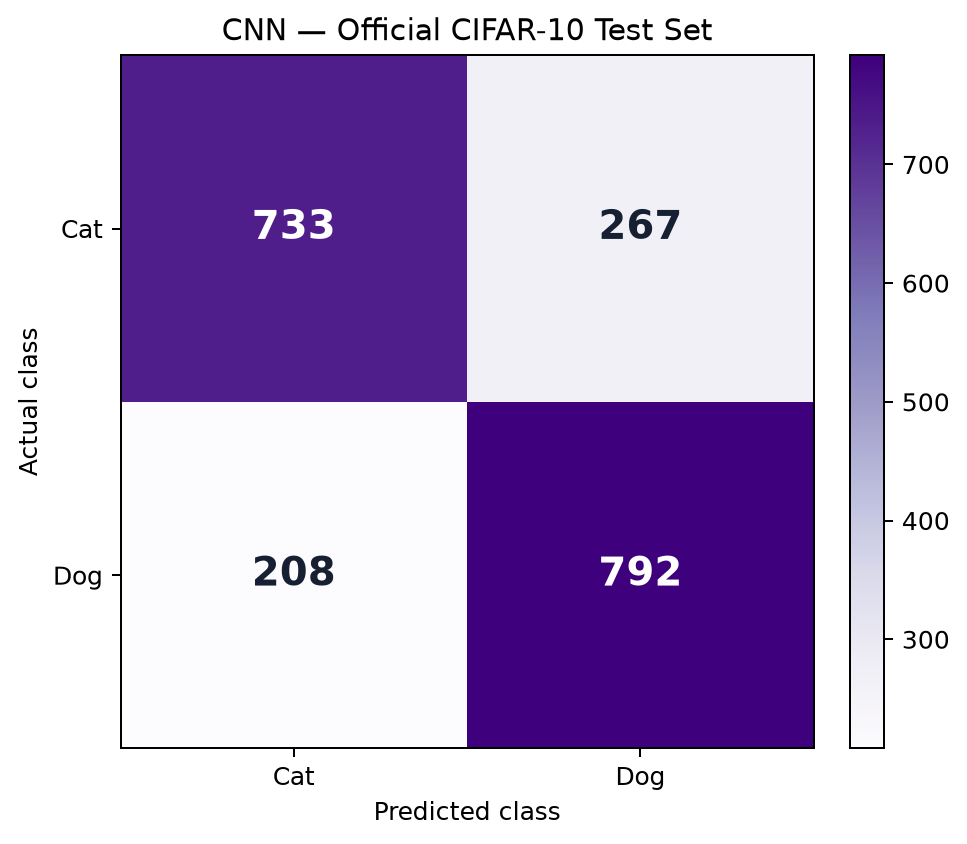
\includegraphics[width=0.80\textwidth]{figures/cnn_confusion.png}
\caption{CNN confusion matrix for 1,000 cat and 1,000 dog test images.}
\label{fig:cnncm}
\end{figure}

\begin{table}[H]\centering
\caption{Consecutive external-image predictions}
\begin{tabular}{lcc}\toprule
Input&Prediction&Confidence\\\midrule
Sample cat image&Cat&98.05\%\\
Sample dog image&Dog&77.99\%\\\bottomrule
\end{tabular}\end{table}

\section{Discussion}
The model correctly classified 733 of 1,000 cats and 792 of 1,000 dogs. Dog recall was therefore higher than cat recall on this test subset. The total accuracy of 76.25\% is substantially above random binary classification but leaves 475 errors, so confidence values must not be treated as guarantees.

Specifically, 267 cats were labelled Dog and 208 dogs were labelled Cat. A confidence such as 98.05\% describes the model output for that single image; it does not mean that the model is 98.05\% accurate in general.

CIFAR-10 images are only $32\times32$ pixels and differ from high-resolution photographs. Resizing an external photograph does not remove this domain difference. Data augmentation, batch normalisation, a larger domain-matched dataset, or transfer learning could improve generalisation. The consecutive sample test confirmed that the interface refreshed its image and prediction state correctly.

\section{Conclusion}
The CNN experiment completed dataset preparation, convolutional feature learning, validation-aware training, official-test evaluation, model saving, and repeated external-image inference. The trained model achieved 76.25\% test accuracy while retaining clearly stated limitations.

\end{document}
